% !TeX spellcheck = en_US	


\documentclass[10pt,journal,compsoc]{IEEEtran}
\usepackage{graphicx}
\usepackage[ruled, linesnumbered]{algorithm2e}
\usepackage{url}
\usepackage{epstopdf}
\usepackage{indentfirst}
\usepackage[tight,footnotesize]{subfigure}
\usepackage{amsmath}
\usepackage{amssymb}
\usepackage{multirow}
\usepackage{color}
\usepackage{enumerate}

\newtheorem{Formula}{Formula}
\newtheorem{Lemma}{Lemma}
\newtheorem{Corollary}{Corollary}
\newtheorem{Property}{Property}
\newtheorem{Rule}{Rule}

% *** CITATION PACKAGES ***
\ifCLASSOPTIONcompsoc
\usepackage[nocompress]{cite}
\else
\usepackage{cite}
\fi


\begin{document}


\title{Checking Big Suffix and LCP Arrays by Probabilistic Methods}

\author{
	Yi~Wu,
	Ge~Nong,
	Wai~Hong~Chan,
	Ling~Bo~Han% <-this % stops a space
	\IEEEcompsocitemizethanks{
		\IEEEcompsocthanksitem Y. Wu, G. Nong (corresponding author) and L.~B.~Han are with the Department of Computer Science, Sun Yat-sen University, Guangzhou, and the SYSU-CMU Shunde International Joint Research Institute, Shunde, China. E-mails: wu.yi.christian@gmail.com, issng@mail.sysu.edu.cn, hanlb@mail2.sysu.edu.cn.
		
		\IEEEcompsocthanksitem Wai Hong Chan (corresponding author) is with the Department of Mathematics and Information Technology, The Education University of Hong Kong, Hong Kong. E-mail: waihchan@ied.edu.hk.
}}% <-this % stops a space
	
\IEEEtitleabstractindextext{%
\begin{abstract}

For full-text indexing of massive data, the suffix and LCP (longest common prefix) arrays have been recognized as fundamental data structures, and there are at least two needs in practice for checking their correctness, i.e. program debugging and verifying the arrays constructed by probabilistic algorithms. Two probabilistic methods are proposed to check the suffix and LCP arrays of constant or integer alphabets in external memory using a Karp-Rabin fingerprinting technique, where the checking  is wrong only with a negligible error probability. The first method checks the lexicographical order and the LCP-value of two suffixes by computing and comparing the fingerprints of their LCPs. This method is general in terms of that it can verify any full or sparse suffix/LCP array of any order. The second method uses less space, it first employs the fingerprinting technique to verify a subset of the given suffix and LCP arrays, from which two new suffix and LCP arrays are induced and compared with the given arrays for verification, where the induced suffix and LCP arrays can be removed for constant alphabets to save space.

\end{abstract}

% Note that keywords are not normally used for peerreview papers.
\begin{IEEEkeywords}
	Suffix and LCP arrays, verification, Karp-Rabin fingerprinting, external memory.
\end{IEEEkeywords}}


% make the title area
\maketitle

\IEEEdisplaynontitleabstractindextext

\IEEEpeerreviewmaketitle

\section{Introduction}\label{sec:introduction}

\subsection{Background} \label{sec:introduction:background}

Suffix and longest common prefix (LCP) arrays play an important role in various string processing tasks, such as data compression, pattern matching and genome assembly. In many applications, these two data structures make up the core part of a powerful full-text index, called enhanced suffix array~\cite{Abouelhodaa2004}, which is more space efficient than a suffix tree and applicable to emulating most searching functionalities provided by the latter in the same time complexity. The first algorithm for building suffix array~(SA) in internal memory was presented in~\cite{Manber1993}. From then on, much more effort has been put on designing efficient constructors for suffix array on different computation models~\cite{Karkkainen2003, Ko2003, Kim2003, Nong11, Dementiev2008, Ferragina2012, Manzini2004, Bingmann12, Karkkainen2014, Nong14, Nong15}. In respect of the research on LCP array construction algorithms, the existing works can be classified into two categories with regard to their input requirements, where the algorithms from the first category compute both suffix and LCP arrays at the same time with the original text only~\cite{Fischer11, Bingmann12, Flick2015}, and those from the second category carry out the computation by taking SA and/or Burrows-Wheeler transform (BWT) as additional inputs~\cite{Kasai2001,Karkkainen2009, Fischer11, Puglisi2008, Deo2013}. So far, the algorithms designed by the induced sorting~(IS) principle take linear time and space to run and get the best results on both internal and external memory~\cite{Nong11, Bingmann12}. In addition to the sequential algorithms, there are also parallel algorithms proposed to achieve high performance by fully using the available multi-core CPUs and/or GPUs~\cite{Osipov2012, Deo2013, Wang2015, Karkkainen2015, Karkkainen2016}.

While the research on efficient construction of suffix and LCP arrays keeps evolving, the algorithms proposed recently are becoming more complicated than before. Currently, the open source programs for the state-of-the-art algorithms are provided "as-is" for demonstration and experiment purpose only, giving no guarantee that they have correctly implemented the algorithms. As a common practice, a suffix or LCP checker is provided to check the correctness of a constructed array. For example, such a checker can be found in some software packages for DC3~\cite{Dementiev08}, SA-IS~\cite{Nong11}, eSAIS~\cite{Bingmann12} and so forth. In addition to help avoid implementation bugs, a checker is also demanded for an array constructed by a probabilistic algorithm~(e.g.~\cite{Bille2013}). In this case, the array is correctly constructed with a probability and hence must be verified by a checker to ensure its correctness. As far as we know, the work in~\cite{Burkhardt2003} describes the only SA checking method that can be found in the existing literature, and no efficient checking method for LCP array has been reported yet. Particularly, there is currently no reported solution that can check both the suffix and the LCP arrays in external memory. This motivates our work here to design efficient checkers for big suffix and LCP arrays in external memory.  

	
\subsection{Contribution}\label{sec:introduction:contribution}

Our contribution comprises two methods to probabilistically verify any given suffix and LCP arrays. In principle, Method A checks the lexical order and the LCP-value of two neighboring suffixes in the suffix array by literally comparing the characters of their LCPs. For reducing the time complexity of a comparison between two sequences of characters, we use a Karp-Rabin fingerprinting technique to convert each sequence into a single integer, called fingerprint, and compare the fingerprints instead to check the equality of two sequences. The algorithm for Method A involves multiple scans and sorts on sets of $\mathcal{O}(n)$ fixed-size items. Its implementation in external memory suffers from a space bottleneck due to the large disk volume taken by each sort. 
To overcome this drawback, Method B first employs the fingerprinting technique to check a subset selected from the given suffix and LCP arrays, 
%then it reuses the inducing process of the IS-based construction algorithm SA-IS \cite{Nong11} to produce the final suffix and LCP arrays from the verified subset and literally compares them with the input arrays to ensure the correctness of the latter. Our experiments indicate that the peak disk use of the programs for Algorithm~\ref{alg:2} designed by Method B is only about half as that of the program for Algorithm~\ref{alg:1} designed by Method A. 
then it utilizes the IS method to produce the final suffix and LCP arrays from the verified subset and literally compares them with the input arrays to ensure the correctness of the latter. Our experiments indicate that the program for Algorithm~\ref{alg:2} designed by Method B only takes around half as much disk space as the program for Algorithm~\ref{alg:1} designed by Method A.

The remainder of this paper is organized as follows. Sections~\ref{sec:method1} and~\ref{sec:method2} describe the two methods and their algorithmic designs. Section~\ref{sec:experiment} conducts an experimental study for performance evaluation of our programs for these algorithms. Finally, Section~\ref{sec:conclusion} gives some concluding remarks.

\section{Method A} \label{sec:method1}


\subsection{Preliminaries} \label{sec:method1:notations}

Given a string $x[0, n-1]$ drawn from a constant or integer alphabet $\Sigma$ of size $\mathcal{O}(1)$ or $\mathcal{O}(n)$, respectively, the suffix array of $x$, denoted by $sa$, is a permutation of $\{0, 1, ..., n - 1\}$ such that ${\sf suf}(sa[i]) < {\sf suf}(sa[j])$ for $i, j \in [0, n)$ and $i < j$, where ${\sf suf}(sa[i])$ and ${\sf suf}(sa[j])$ are two suffixes starting with $x[sa[i]]$ and $x[sa[j]]$, respectively. Particularly, we say ${\sf suf}(sa[j])$ is a lexical neighbor of ${\sf suf}(sa[i])$ if $|i - j| = 1$. The LCP array of $x$, denoted by $lcp$, consists of $n$ integers, where $lcp[0]=0$ and $lcp[i]$ records the LCP-value of ${\sf suf}(sa[i])$ and ${\sf suf}(sa[i - 1])$ for $i \in [1, n)$. A suffix/LCP array is infinite-order if the suffixes/LCPs are sorted/counted up to their ends, respectively, or else finite-order.

\subsection{Idea} \label{sec:method1:idea}

According to the above definitions, we give in Lemma~\ref{lemma:1} the sufficient and necessary conditions for checking both suffix and LCP arrays. Notice that the lexical order and the LCP-value of any two suffixes in $x$ can be computed by literally comparing their characters. For convenience, we append a virtual character to $x$ and assume it to be lexicographically smaller than any characters in $\Sigma$, hence any two suffixes are different.


\begin{Lemma} \label{lemma:1}
	Both $sa[0, n)$ and $lcp[0, n)$ are correct if and only if the following conditions are satisfied, for all $i \in [1, n)$:
	\begin{enumerate}[(1)]
		\item
		$sa$ is a permutation of $\{0, 1, \dots, n - 1\}$.
		\item
		$x[sa[i], sa[i] + lcp[i] - 1] = x[sa[i - 1], sa[i - 1] + lcp[i] - 1]$.
		\item
		$x[sa[i] + lcp[i]] > x[sa[i - 1] + lcp[i]]$. 	
	\end{enumerate}
\end{Lemma}

\begin{IEEEproof}
	Both the sufficiency and necessity are immediately from the definitions of suffix and LCP arrays. Condition 1 guarantees that each suffix is in $sa$, conditions 2 and 3 guarantees that the lexical order and the LCP-value of any two neighboring suffixes in $sa$ are both correct.
\end{IEEEproof}

Directly comparing the characters of two suffixes to determine their LCP has the worst case time of $O(n)$. An alternative is to exploit a perfect hash function to convert each substring into a single integer such that any two substrings have a common hash value if and only if they are literally equal to each other, hence the hash values of two substrings can be compared instead to check the equality of two substrings. Taking into account the high difficulty of finding a perfect hash function to meet this requirement, we prefer using a Karp-Rabin fingerprinting function~\cite{Karp1987} to transform a substring into an integer called fingerprint. To be specific, suppose $L$ is a prime and $\delta$ is a number randomly chosen from $[1, L)$, the fingerprint ${\sf fp}(i, j)$ for a substring $x[i, j]$ can be iteratively calculated according to the formulas below: scan $x$ rightward to iteratively compute ${\sf fp}(0, k)$ for all $k \in [0, n)$ using Formulas~\ref{formula:1}-\ref{formula:2}, record ${\sf fp}(0, i - 1)$ and ${\sf fp}(0, j)$ during the calculation and subtract the former from the latter to obtain ${\sf fp}(i, j)$ using Formula~\ref{formula:3}.


\begin{Formula} \label{formula:1}
	${\sf fp}(0, -1) = 0$.
	
\end{Formula}

\begin{Formula} \label{formula:2}	
	${\sf fp}(0, i) = {\sf fp}(0, i - 1) \cdot {\delta} + x[i]\mod L$ for $i \ge 0$.
	
\end{Formula}

\begin{Formula} \label{formula:3}
	${\sf fp}(i, j) = {\sf fp}(0, j) - {\sf fp}(0 ,i - 1) \cdot {\delta}^{j - i + 1}\mod L$.
	
\end{Formula}


Notice that two equal substrings always share a common fingerprint, but the inverse is not true. The probability of a false match can be reduced to a negligible level by setting $L$ to a large value~\cite{Karp1987}, this property is utilized in~\cite{Bille2013} to design a probabilistic algorithm for computing a sparse suffix array. Hence we have:


\begin{Corollary} \label{corollary:1}
	Both $sa[0, n)$ and $lcp[0, n)$ are correct with a high probability given these conditions, for all $i \in [1, n)$:
	
	\begin{enumerate}[(1)]
		\item
		$sa$ is a permutation of $\{0, 1, \dots, n - 1\}$.
		
		\item
		${\sf fp}(sa[i], sa[i] + lcp[i] - 1) = {\sf fp}(sa[i - 1], sa[i - 1] + lcp[i] - 1)$.
		
		\item
		$x[sa[i] + lcp[i]] > x[sa[i - 1] + lcp[i]]$.
	\end{enumerate}
\end{Corollary}

Fig.~\ref{fig:example} gives an illustrating example for utilizing Corollary~\ref{corollary:1} to check the input suffix and LCP arrays. Given that $L = 197$ and $\delta = 101$, lines 4-8 compute ${\sf fp}(0, p)$ iteratively according to Formulas~\ref{formula:1}-\ref{formula:2}. Lines 10-20 use these values to compute the fingerprints for all the target substrings. In more detail, consider the leftmost pair of neighboring suffixes in $sa$, i.e. ${\sf suf}(sa[0])$ and ${\sf suf}(sa[1])$, the substrings given by their LCP-value are $x[sa[0], sa[0] + lcp[1] - 1]$ and $x[sa[1], sa[1] + lcp[1] - 1]$, respectively. According to Formula~\ref{formula:3}, ${\sf fp}(sa[0], sa[0] + lcp[1] - 1)$ is equal to the difference between ${\sf fp}(0, sa[0] - 1)$ and ${\sf fp}(0, sa[0] + lcp[1] - 1)$, both have been calculated. Following the same way, ${\sf fp}(sa[1], sa[1] + lcp[1] - 1)$ is computed by reducing ${\sf fp}(0, sa[1] - 1)$ from ${\sf fp}(0, sa[1] + lcp[1] - 1)$. Hence, we obtain the fingerprints for these two substrings in lines 10-14 and see that they are equal to each other.

\begin{figure}
	\centering
	
	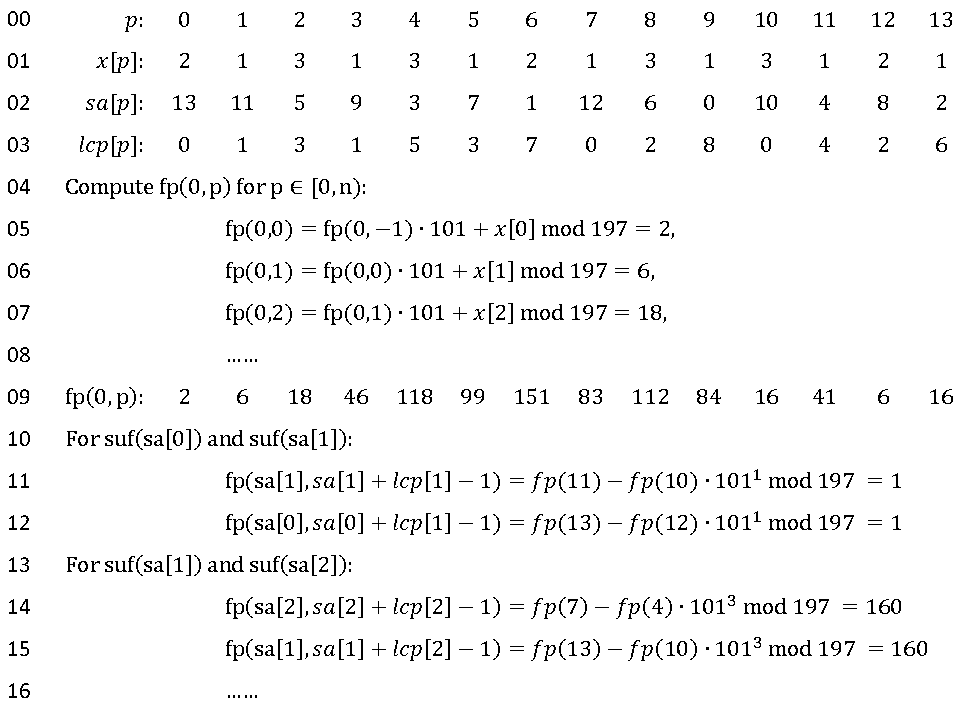
\includegraphics[width = 0.9\columnwidth]{example}
	\caption{An example for computing and comparing fingerprints for substrings specified by the LCP-values of neighboring suffixes in $sa$. \label{fig:example}}	
\end{figure}

\subsection{Algorithm} \label{sec:method1:algorithm}

We describe an approach for checking the conditions in Corollary~\ref{corollary:1} on random access models, of which the core part is to check the lexical order and the LCP-value for each pair of neighboring suffixes in $sa$ during the scan of $sa$ and $lcp$. This is done by using Formulas~\ref{formula:1}-\ref{formula:3}. Two zero-initialized arrays $fp$ and $mk$ are introduced to facilitate the checking process, where $fp$ is for storing the fingerprints of all the prefixes in $x$ and $mk$ is for checking whether $sa$ stores a permutation of $\{0, 1, ..., n - 1\}$.

\begin{enumerate}
	\item [S1]
	Scan $x$ with $i$ increasing from $0$ to $n - 1$, for each scanned $x[i]$, compute ${\sf fp}(0, i)$ and assign to $fp[i]$.
	
	\item [S2]
	Scan $sa$ and $lcp$ with $i$ increasing from $1$ to $n - 1$, for each scanned $sa[i]$ and $lcp[i]$, let $u = sa[i], v = lcp[i]$ and $w = sa[i - 1]$, perform:
	
	\begin{enumerate}[(a)]
		\item
		Retrieve $fp[u - 1]$ and $fp[u + v - 1]$ from $fp$ to compute ${\sf fp}(u, u + v - 1)$, set $mk[u]=1$;
		
		\item
		Retrieve $fp[w - 1]$ and $fp[w + v - 1]$ from $fp$ to compute ${\sf fp}(w, w + v - 1)$;
		
		\item
		Check if ${\sf fp}(u, u + v - 1) = {\sf fp}(w, w + v - 1)$ and $x[u + v] > x[w + v]$;
		
		\item
		Set $mk[sa[0]] = 1$.
	\end{enumerate}

	\item [S3] Check if $mk[i] = 1$ for all $i \in [0, n)$.
	
\end{enumerate}

The above approach takes $\mathcal{O}(n)$ time and space in internal memory. The difficulty for applying it in external memory is step S2, it suffers from a performance degradation caused by frequent random accesses to disks. Assume that $x$, $sa$ and $lcp$ are stored in external memory, we design Algorithm~\ref{alg:1} for conducting these I/O operations in a disk-friendly way. The idea is to first sort data in the order that they are to be visited and then access them sequentially. For this purpose, Algorithm~\ref{alg:1} first scans $sa$ and $lcp$ to produce $ST_1, ST_2, ST_3$, and sorts their tuples by the first components in ascending order at the beginning (lines~\ref{alg:1:a}-\ref{alg:1:b}). Afterward, it iteratively computes the fingerprints of all the prefixes of $x$ according to Formulas~\ref{formula:1}-\ref{formula:2} and assigns them to the sorted tuples as follows (lines~\ref{alg:1:c}-\ref{alg:1:d}): when figuring out ${\sf fp}(0, i - 1)$, extract each tuple $e$ with $e.1st = i$ from $ST_1/ST_2/ST_3$, update $e$  with ${\sf fp}(0, i - 1)$, and then forward $e$ to $ST_1'/ST_2'/ST_3'$. Because the first components of the tuples in $ST_1$ constitute a copy of $sa$, the algorithm checks condition 1 when scanning these tuples in their sorted order. Finally, it sorts the updated tuples back to their original order~(line~\ref{alg:1:e}) and visits them sequentially to check conditions 2 and 3 following the same way of step S2~(lines~\ref{alg:1:f}-\ref{alg:1:g}).  



\SetKwProg{Fn}{Function}{}{}

\begin{algorithm*}

	\caption{The Algorithm Based on Corollary~\ref{corollary:1}.}
	
	\label{alg:1}
	
	%\SetAlgoNoLine
	\Fn{{\sf CheckByFP}($x$, $sa$, $lcp$, $n$)}{
	
		$ST_1$ := $[(sa[i], i, null) | i \in [0, n)]$ \label{alg:1:a}
		
		$ST_2$ := $[(sa[i] + lcp[i + 1], i, null, null) | i \in [0, n - 1)]$
			
		$ST_3$ := $[(sa[i] + lcp[i], i, null, null) | i \in [1, n)]$
		
		sort the tuples in $ST_1$, $ST_2$ and $ST_3$ by the 1st components, respectively; \label{alg:1:b}
		
		$fp := 0$  \label{alg:1:c}
		
		\For{$i \in [0, n]$}{
			
			\If{$ST_1.{\sf notEmpty}()$ {\sf and} $ST_1.{\sf top}().1st = i$}{~\label{alg:1:h}
				$e := ST_1.{\sf top}()$, $ST_1.{\sf pop}()$, $e.3rd := fp$, $ST_1'.{\sf push}(e)$
			}
			\Else{
				\Return false \hspace{1cm} // condition 1 is violated
			}~\label{alg:1:i}
			\While{$ST_2.{\sf notEmpty}()$ {\sf and} $ST_2.{\sf top}().1st = i$}{
				
				$e := ST_2.{\sf top}()$, $ST_2.{\sf pop}()$, $e.3rd := fp$, $e.4th := x[i]$, $ST_2'.{\sf push}(e)$
			}	
		
			\While{$ST_3.{\sf notEmpty}()$ {\sf and} $ST_3.{\sf top}().1st = i$}{
				
				$e := ST_3.{\sf top}()$, $ST_3.{\sf pop}()$, $e.3rd := fp$, $e.4th := x[i]$, $ST_3'.{\sf push}(e)$
			}	
		
			$fp := fp \cdot \delta + x[i] \! \mod \! P$ \hspace{1cm} // $x[n]$ is the virtual character
		} \label{alg:1:d}
		
		sort the tuples in $ST_1'$, $ST_2'$ and $ST_3'$ by the 2nd component, respectively; \label{alg:1:e}
		
		\For {$i \in [1, n)$}{  \label{alg:1:f}
			
			$fp_1 := ST_1'.{\sf top}().3rd$, $ST_1'.{\sf pop}()$, $fp_2 := ST_2'.{\sf top}().3rd$, $ch_1 := ST_2'.{\sf top}().4th$, $ST_2'.{\sf pop}()$
			
			$\hat{fp_1} = fp_2 - fp_1 \cdot \delta^{lcp[i]} \! \mod \! P$ \label{alg:1:j}
		
		 	$fp_1 := ST_1'.{\sf top}().3rd$, $fp_3 := ST_3'.{\sf top}().3rd$, $ch_2 := ST_3'.{\sf top}().4th$, $ST_3'.{\sf pop}()$
			
			$\hat{fp_2} = fp_3 - fp_1 \cdot \delta^{lcp[i]} \! \mod \! P$	\label{alg:1:k}
			
			\If{$\hat{fp_1} \ne \hat{fp_2}$ {\sf or} $ch_1 \ge ch_2$}{
				
				\Return false \hspace{1cm} // condition 2 or 3 is violated
			}	
		} \label{alg:1:g}

		\Return true
	}
\end{algorithm*}

The last point is how to obtain $\delta^{lcp[i]}$ quickly when computing $\hat{fp_1}$ and $\hat{fp_2}$ in lines~\ref{alg:1:j} and~\ref{alg:1:k}. One way is to keep a lookup table in internal memory to store all $\delta^{lcp[i]}$. This can answer the question in constant time, but it is space-consuming and impractical to be used in external memory. Notice that the LCP of any two suffixes is shorter than $n$, we can return the answer in $\mathcal{O}(\lceil \log_2{n} \rceil)$ time using $\mathcal{O}(\lceil \log_2{n} \rceil)$ internal memory. Let $e$ be an integer from $[0, n)$, its binary form is $k_{\lceil \log_2{n} \rceil}...k_1k_0$. We have $\delta^e = \Pi_{i = 0}^{\lceil \log_2{n} \rceil}{\delta}^{k_i \cdot 2^i}$, which can be computed with $\{{\delta}^{1}, {\delta}^{2}, \dots, {\delta}^{2^{\lceil \log_2{n} \rceil}} \}$ already known.

\subsection{Analysis} \label{sec:method1:analysis}


Algorithm~\ref{alg:1} performs multiple scans and sorts on the arrays of $\mathcal{O}(n)$ fixed-size tuples in disks. Given RAM size $M$, disk size $D$ and block size $B$, all are in words, the time and I/O complexities for each scan are $\mathcal{O}(n)$ and $\mathcal{O}(n / B)$, respectively, while those for each sort are $\mathcal{O}(n\log_{M/ B}(n / B))$ and $\mathcal{O}((n / B)\log_{M / B}(n / B))$, respectively~\cite{Arge2013}. Algorithm~\ref{alg:1} reaches its peak disk use when sorting the tuples in lines~\ref{alg:1:b} and~\ref{alg:1:e}. Suppose the input string and the suffix/LCP array are encoded as $\alpha$- and $\beta$-byte integers, respectively, and each fingerprint is a $\gamma$-byte integer, it takes $(2 \cdot \beta + \gamma)$ space for sorting the tuples of $ST_1/ST_1'$ and $(\alpha + 2 \cdot \beta + \gamma)$ for sorting the tuples of $ST_2/ST_2'$ and $ST_3/ST_3'$. For saving space, our program implementing the algorithm tackles $ST_1/ST_1'$, $ST_2/ST_2'$ and $ST_3/ST_3'$ separately and performs a single scan over $x$ for each of them to obtain the fingerprints, using less space but more time. The experiment in Section~\ref{sec:experiment} indicates that the disk use is 40 times of $x$.

\section{Method B} \label{sec:method2}

\subsection{Preliminaries} \label{sec:method2:preliminaries}

We further to give another checking method using the induced sorting principle \cite{Nong11,Dementiev08}, which requires much less space than Method A. For presentation convenience, we introduce some symbols and notations as below.

Character and suffix classification. All the characters in $x$ are classified into three types, namely L-, S- and S*-type. In detail, $x[i]$ is L-type if (1) $i = n - 1$ or (2) $x[i] > x[i + 1]$ or (3) $x[i] = x[i + 1]$ and $x[i + 1]$ is L-type; otherwise, $x[i]$ is S-type. Further, if $x[i]$ and $x[i + 1]$ are separately L-type and S-type, then $x[i + 1]$ is also S*-type. Moreover, a suffix is L-, S- or S*-type if its heading character is L-, S-, or S*-type, respectively.

Suffix and LCP buckets. All the suffixes in $sa$ are partitioned into multiple buckets and those of a common heading character are grouped into a single bucket that occupies a contiguous interval in $sa$. Each bucket can be further divided into two sub-buckets, where the left and the right parts  contain L- and S-type suffixes only, respectively. For short, we use ${\sf sa\_bkt}(c)$ to denote the bucket storing the suffixes starting with character $c$ and ${\sf sa\_bkt_L}(c)/{\sf sa\_bkt_S}(c)$ to denote its left/right sub-bucket. Accordingly, $lcp$ can be also split into multiple buckets, where ${\sf lcp\_bkt}(c)/{\sf lcp\_bkt_L}(c)/{\sf lcp\_bkt_S}(c)$ stores the LCP-values of suffixes in ${\sf sa\_bkt}(c)/{\sf sa\_bkt_L}(c)/{\sf sa\_bkt_S}(c)$, respectively.

Suffix and LCP arrays for S*-type suffixes. Given that the number of S*-type suffixes is $n_1$, $sa^*[0, n_1)$ stores all the S*-type suffixes arranged in lexical order, while $lcp^*[0] = 0$ and $lcp^*[i]$ records the LCP-value of ${\sf suf}(sa^*[i])$ and ${\sf suf}(sa^*[i - 1])$ for $i \in [1, n_1)$.

Type Array. The array $t$ records in $t[i]$ the type information of $x[i]$, where $t[i] = 1$ or $0$ if $x[i]$ is S- or L-type, respectively.

\subsection{Idea} \label{sec:method2:idea}

The induced sorting principle has been extensively used to design efficient algorithms for constructing the suffix and LCP arrays in internal or external memory \cite{Nong11,Nong14, Nong15, Bingmann12,Fischer11}. Such a construction algorithm mainly consists of a reduction phase for computing $sa^*$ and $lcp^*$, followed by an induction phase for inducing $sa$ and $lcp$ from $sa^*$ and $lcp^*$~\footnote{An overview of the induction phase is given in Appendix~\ref{sec:appendix}.}. Given that $sa^*$ and $lcp^*$ are already known, we can induce the final suffix and LCP arrays from them. This suggests a checking method based on Lemma~\ref{lemma:2}. 
	
\begin{Lemma} \label{lemma:2}
Both $sa[0, n)$ and $lcp[0, n)$ are correct if and only if the conditions below are satisfied:

\begin{enumerate}[(1)]
	\item
	Both $sa^*$ and $lcp^*$ are correct.
	\item
	$sa = sa'$ and $lcp = lcp'$, where $sa'$ and $lcp'$ are induced from $sa^*$ and $lcp^*$ by the IS method.
\end{enumerate}
\end{Lemma}

We have Corollary~\ref{corollary:2} for probabilistically checking the conditions of Lemma \ref{lemma:2}.

\begin{Corollary} \label{corollary:2}
Both $sa[0, n)$ and $lcp[0, n)$ are correct with a high probability given the following conditions, for all $i \in [1, n_1)$ and $j \in [0, n)$:
\begin{enumerate}[(1)]
	\item
	$x[sa^*[i]]$ is S*-type, and $sa^*[i] \ne sa^*[k]$ for all $k \in [0, n_1)$ and $k \ne i$.
	\item
	${\sf fp}(sa^*[i], sa^*[i] + lcp^*[i] - 1) = {\sf fp}(sa^*[i - 1], sa^*[i - 1] + lcp^*[i] - 1)$.
	\item
	$x[sa^*[i] + lcp^*[i]] > x[sa^*[i - 1] + lcp^*[i]]$.
	\item
	$sa[j] = sa'[j]$ and $lcp[j] = lcp'[j]$ for $j \in [0, n)$, where $sa'$ and $lcp'$ are induced from $sa^*$ and $lcp^*$ by the IS method.
\end{enumerate}
\end{Corollary}



\subsection{Algorithm} \label{sec:method2:algorithm}

We further to design Algorithm~\ref{alg:2} for checking the conditions of Corollary~\ref{corollary:2}. The first step is to compute and verify $sa^*$ and $lcp^*$. Similar to Method A, the fingerprinting technique is employed to probabilistically check the correctness of $sa^*$ and $lcp^*$.  The array $sa^*$ can be produced by sequentially retrieving the S*-type suffixes from $sa$ and the LCP-value of two successive S*-type suffixes in $sa$, say ${\sf suf}(sa[i])$ and ${\sf suf}(sa[j])$, is equal to the minimal of $\{lcp[i + 1], ..., lcp[j - 1], lcp[j]\}$. The algorithm first sorts all the suffixes in $sa$ by their starting positions~(lines~\ref{alg:2:a}-\ref{alg:2:b}) and then scans $x$ once to get the S*-type suffixes~(lines~\ref{alg:2:c}-\ref{alg:2:d}). After that, it puts these S*-type suffixes back in their lexical order and outputs them one by one to generate $sa^*$~(lines~\ref{alg:2:g}-\ref{alg:2:h}). Meanwhile, it calculates the LCP-value for each pair of the neighboring suffixes in $sa^*$ by tracing the minimum in the $lcp$ interval between these two suffixes. Notice that, we check condition 1 when visiting the suffixes in their position order (lines~\ref{alg:2:e}-\ref{alg:2:f}), and check conditions 2 and 3 by Algorithm~\ref{alg:1} with $sa^*$ and $lcp^*$ as input. Given $sa^*$ and $lcp^*$ are correct, 
Algorithm~\ref{alg:2} invokes an inducing process by employing the IS method to induce $sa'$ and $lcp'$ from $sa^*$ and $lcp^*$~(line~\ref{alg:2:k}) and compares them with $sa$ and $lcp$ to complete the whole checking process~(lines~\ref{alg:2:l}-\ref{alg:2:m}).

\begin{algorithm*}[!htbp]
	
	\caption{The Algorithm Based on Corollary~\ref{corollary:2}.}
	
	\label{alg:2}
	
	%\SetAlgoNoLine
	\Fn{{\sf CheckByIS}($x$, $sa$, $lcp$, $n$)}{	
	
	$ST_1$ := $[(sa[i], i, null) | i \in [0, n)]$ \label{alg:2:a}
		
	sort the tuples in $ST_1$ by the 1st component; \label{alg:2:b}
	
	$pos := -1$ \label{alg:2:c}
	
	\For{$i \in (n, 0]$}{
	
		$e := ST_1.{\sf top}()$, $ST_1.{\sf pop}()$
		
		\If{$x[i]$ is S*-type}{ \label{alg:2:e}
			
			\If{$pos \ge e.1st$}{
			
				\Return false  \hspace{1cm} // condition 1 is violated
			}
		
			$ST_2.{\sf push}(e)$, $pos := e.1st$
		}\label{alg:2:f}
	} \label{alg:2:d}

	sort the tuples in $ST_2$ by the 2nd component; \label{alg:2:g}
	
	$i := 0$, $j := 0$, $lcp_{min} := max\_val$
	
	\While{$ST_2.{\sf NotEmpty()}$}{
	
		$e := ST_2.{\sf top}()$, $ST_2.{\sf pop}()$
	
		\While {true} {
			
			$lcp_{min} := {\sf min}(lcp_{min}, lcp[i])$
			
			\If {$e.2nd = i$} {
			
				$sa^*[j] := e.1st$, $lcp^*[j] := lcp_{min}$, $j := j + 1$, $i:= i + 1$
				
				\textbf{break}
			}
			
			$i:= i + 1$
		}
	
		$lcp_{min} := max\_val$
	} \label{alg:2:h}
	
	\If{${\sf CheckByFP}(x, sa^*, lcp^*, n_1) = false$}{  \label{alg:2:i}
	
		\Return false \hspace{1cm} // conditions 2 or 3 is violated
	}\label{alg:2:j}

	$(sa', lcp') := {\sf InducingProcess}(x, sa^*, lcp^*)$ \label{alg:2:k}
	
	\For{$i \in [0, n)$}{\label{alg:2:l}
	
		\If{$sa[i] \ne sa'[i] \parallel lcp[i] \ne lcp'[i]$}{
		
			\Return false \hspace{1cm}	// condition 4 is violated
		}	
	}\label{alg:2:m}

	\Return true
}
\end{algorithm*}

Assume that the alphabet $\Sigma$ is of size $\mathcal{O}(1)$, we can check $sa$ and $lcp$ without storing the induced suffix and LCP arrays in Algorithm~\ref{alg:2}. The idea is to compare the induced suffix/LCP items with their corresponding items in $sa/lcp$ during the inducing process. Specifically, when a suffix/LCP item $v_1$ is induced into a bucket, we check if it is equal to the corresponding item $v_2$ in $sa/lcp$. If $v_1 = v_2$, then $v_2$ is correct and we further use this value to induce the remaining suffix/LCP items. The key point is to quickly retrieve the items of $sa/lcp$ in external memory. This can be done by conducting sequential I/O operations if we provide a read pointer together with a buffer for each suffix/LCP sub-bucket. We describe below more details of the modified inducing process, where $lp_1/lp_2$ and $sp_1/sp_2$ indicate the next items to be visited in the L-type and S-type sub-buckets, respectively.

\begin{enumerate}
	\item [S1]
	\begin{enumerate}[(a)]
		\item 
		Let $lp_1[c]$ and $lp_2[c]$ point to the leftmost items of ${\sf sa\_bkt_L}(c)$ and ${\sf lcp\_bkt_L}(c)$, for $c \in [0, \Sigma)$.
		\item 
		Scan $sa$ and $lcp$ rightward to induce the L-type suffixes and their LCP-values. For each induced suffix $p$ (with a heading character $c_0$) and its LCP-value $q$: (1) check if $p = lp_1[c_0]$ and $q = lp_2[c_0]$; (2) move $lp_1[c_0]$ and $lp_2[c_0]$ to the next items on the right.
	\end{enumerate}
	\item [S2]
	\begin{enumerate}[(a)]
		\item 	
		Let $sp_1[c]$ and $sp_2[c]$ point to the rightmost items of ${\sf sa\_bkt_S}(c)$ and ${\sf lcp\_bkt_S}(c)$, for $c \in [0, \Sigma)$.
		\item 	
		Scan $sa$ and $lcp$ leftward to induce the S-type suffixes and their LCP-values. For each induced suffix $p$ (with a heading character $c_0$) and its LCP-value $q$: (1) check if $p = sp_1[c_0]$ and $q = sp_2[c_0]$; (2) move $sp_1[c_0]$ and $sp_2[c_0]$ to the next items on the left.
	\end{enumerate}
\end{enumerate}

\subsection{Analysis} \label{sec:method2:analysis}

Algorithm~\ref{alg:2} mainly consists of two steps, where the first step for checking $sa^*$ and $lcp^*$ can be done within sorting complexity and the second step for checking $sa$ and $lcp$ can also be done in sorting complexity for using external-memory sorters and priority queues. In our current program for this algorithm, the peak disk use is reached in the second step, specifically, when computing the BWT from $sa$ and $x$ for use in the inducing process.

\section{Experiments} \label{sec:experiment}

\subsection{Setup} \label{sec:experiment:setup}

For implementation simplicity, our programs for the algorithms proposed in the previous sections use the external-memory containers provided by the STXXL library~\cite{Dementiev2007} to manage read/write operations on disks. We make a performance evaluation by running them on the real-world corpora listed in Table~\ref{tbl:1}, where three measures normalized by the size of input string are investigated:

\begin{itemize}
	
	\item RT: running time, in microseconds.
	
	\item PDU: peak disk use of external memory, in bytes.
	
	\item IOV: amount of data read from and write to external memory, in bytes, where each integer is 40-bit.
	
\end{itemize}

The experimental platform is a server with an Intel Core i3-550 CPU, 4 GiB RAM and 2 TiB HD. All the programs are compiled by gcc/g++ 4.8.4 with -O3 options on ubuntu 14.04 64-bit operating system and each program is allowed to use 3 GiB RAM. For simplicity, "ProgA" and "ProgB" represent the programs for Algorithms~\ref{alg:1} and~\ref{alg:2}, respectively.

%Table
\renewcommand\arraystretch{1.3}
\begin{table}[!htbp]
	\caption{Corpus, $n$ in Gi, 1 byte per character.}
	\label{tbl:1}
	\centering
	\begin{tabular}{|l|c|c|p{5.2cm}|}
		\hline
		Corpora & \multicolumn{1}{c|}{$\|\Sigma\|$} & $n$ & Description \\\hline
		enwiki & 256 & 74.7 & An XML dump of English Wikipedia, available at \url{https://dumps.wikimedia.org/enwiki}, dated as 16/05/01. \\\hline	
		uniprot & 96 & 2.5 & UniProt Knowledgebase, available at \url{ftp://ftp.expasy.org/databases/uniprot/current_release/knowledgebase/complete/}, dated as 16/05/11. \\\hline
		proteins & 27 & 1.1 & Swissprot database, available at \url{http://pizzachili.dcc.uchile.cl/texts/protein}, dated as 06/12/15. \\\hline
	\end{tabular}
\end{table}


\subsection{Results} \label{sec:experiments:results}

Fig.~\ref{fig:performance_analysis} illustrates the performance comparison of ProgA and ProgB on different datasets, where "enwiki\_8g" consists of the leftmost 8 GiB extracted from "enwiki". As depicted, ProgB runs slower than ProgA by around 20\%. The speed gap is mainly due to the difference in I/O performance. Specifically, the I/O volume of ProgA keeps at $155n$ for all the three datasets, while that of ProgB rises up to nearly $200n$ on average. Besides, the peak disk use of ProgB is about $26/40=0.65$ as ProgA. Recall that Algorithm~\ref{alg:2} invokes Algorithm~\ref{alg:1} to check the suffix and LCP arrays for the S*-type suffixes. Because at most one out of every two successive characters in the input string is S*-type, the consumption for checking the suffix and LCP arrays of S*-type suffixes in ProgB is expected to be half as that for checking the given arrays in ProgA. For a better insight, we collect in Table~\ref{tbl:2} the performance overhead of ProgB and ProgA when checking the suffix and LCP arrays of S*-type suffixes and all, respectively. As can be observed, the mean ratio of the number of S*-type suffixes to the number of all the suffixes is around 0.30 for the datasets under investigation, while the mean ratios of time, space and I/O volume for checking $sa^*$ and $lcp^*$ to that for checking $sa$ and $lcp$ are 0.38, 0.57 and 0.60, respectively. 

The above observations indicate that ProgB reaches its peak disk use when checking the final suffix and LCP arrays during the inducing process, i.e., the inducing process constitutes the performance bottleneck of the whole algorithm. By adopting the space optimization scheme introduced in Section~\ref{sec:method2:algorithm}, we adapt Algorithm~\ref{alg:2} and evaluate the tuned version of ProgB, called ProgB+, in comparison with ProgA and ProgB. Fig.~\ref{fig:performance_analysis} shows that the maximum space requirement for ProgB+ is about $21n$, which is much less than that of ProgB and even only half as that of ProgA. In addition, progB+ outperforms its prototype with respect to time and I/O efficiency and is faster than ProgA when handling "uniprot". We also investigate the performance trend of the three programs on the prefix of "enwiki" with the length varying in $\{1, 2, 4, 8\}$ GiB. In Figure~\ref{fig:performance_analysis2}, the peak disk use for each program remains unchanged, but their speed become slower as the prefix length increases due to the performance degradation of the external memory sorter used in our programs. This can be also observed from Table~\ref{tbl:2}, where ProgB+ keeps the I/O volume around $90n$ with the prefix length of "enwiki" varying from $1$ to $8$ GiB but its running time rises from $1.05$ to $1.33$.


%figure
\begin{figure}
	\centering
	\subfigure{
		\label{subfig:pdu_cmp}
		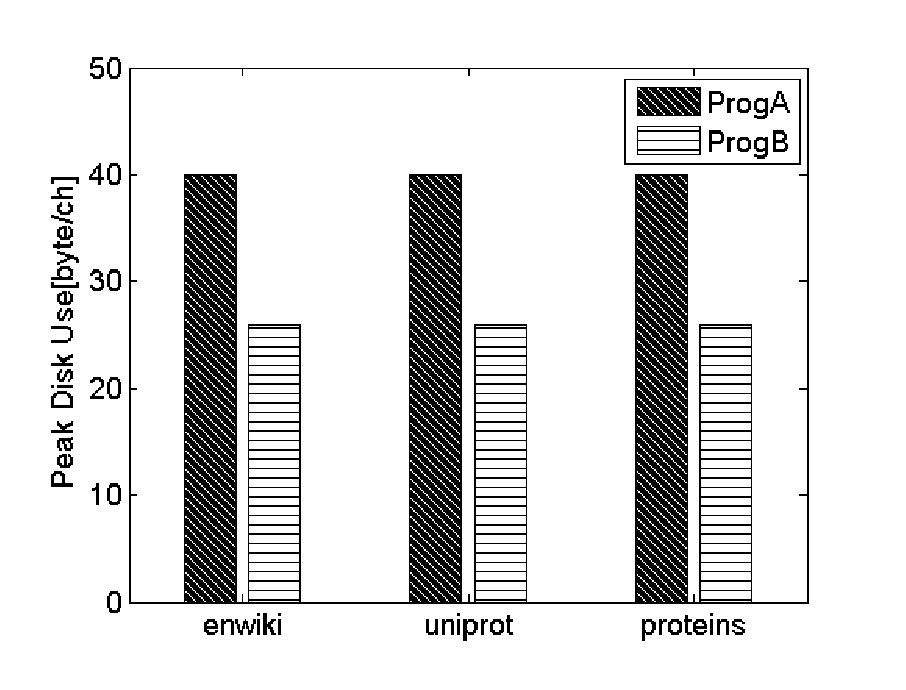
\includegraphics[width = 0.9\columnwidth]{pdu_cmp}
	}
	\hfil
	\subfigure{
		\label{subfig:iov_cmp}
		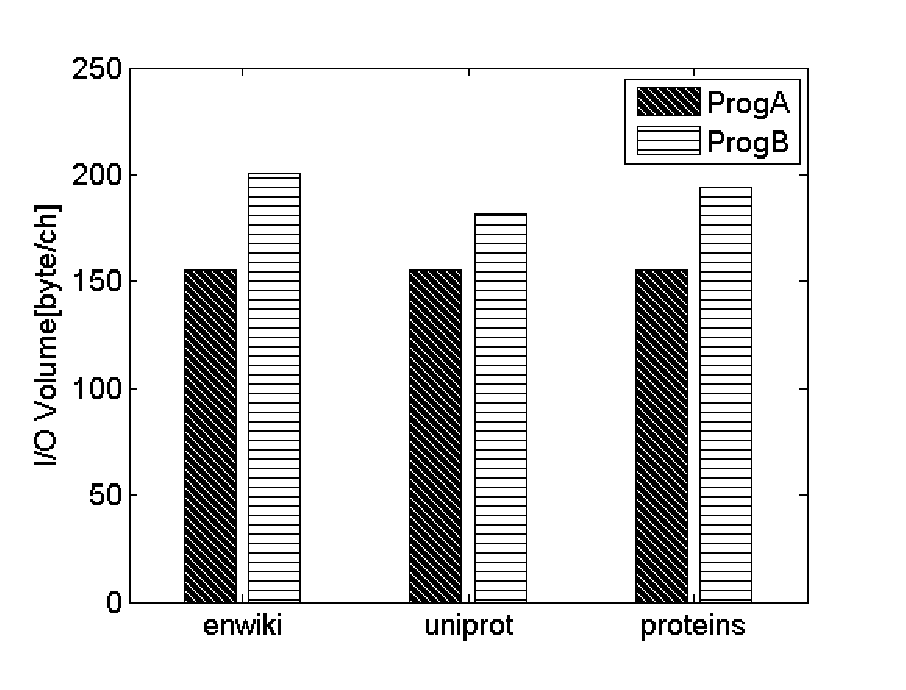
\includegraphics[width = 0.9\columnwidth]{io_cmp}
	}
	\hfil
	\subfigure{
		\label{subfig:ct_cmp}
		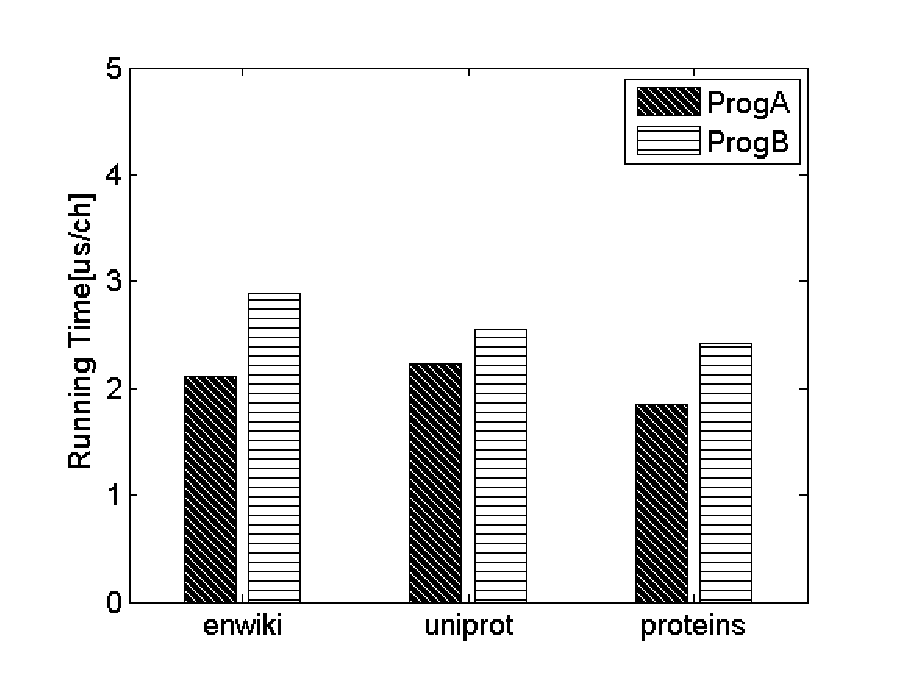
\includegraphics[width = 0.9\columnwidth]{ct_cmp}
	}
	\caption{Performance of ProgA, ProgB, ProgB+ and ProgC for different corpora.}
	\label{fig:performance_analysis}
\end{figure}

%figure
\begin{figure}[htbp!]
	\centering
	\subfigure{
		\label{subfig:pdu_cmp2}
		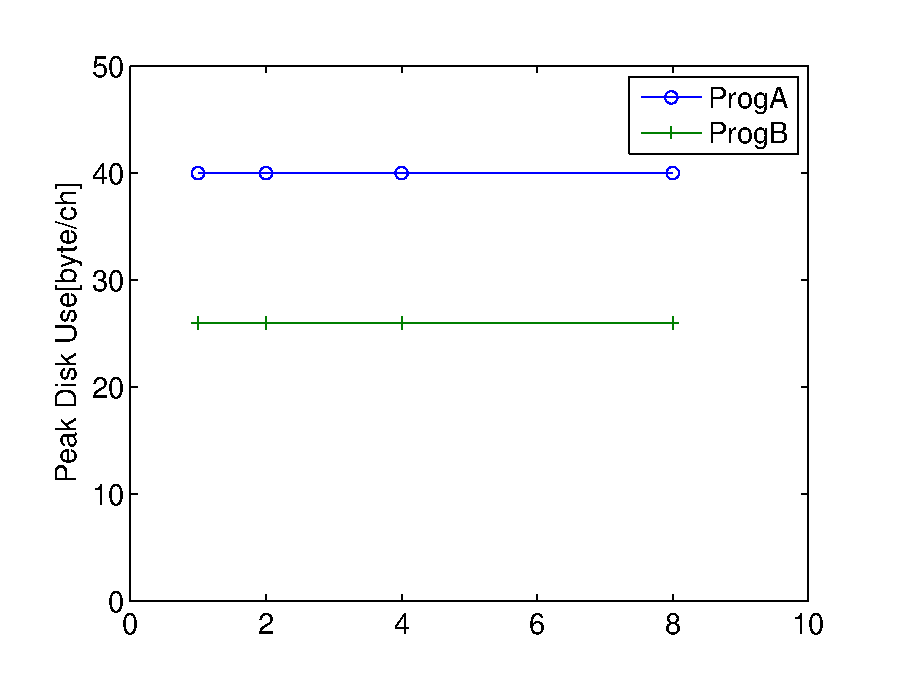
\includegraphics[width = 0.9\columnwidth]{pdu_cmp2}
	}
	\hfil
	\subfigure{
		\label{subfig:iov_cmp2}
		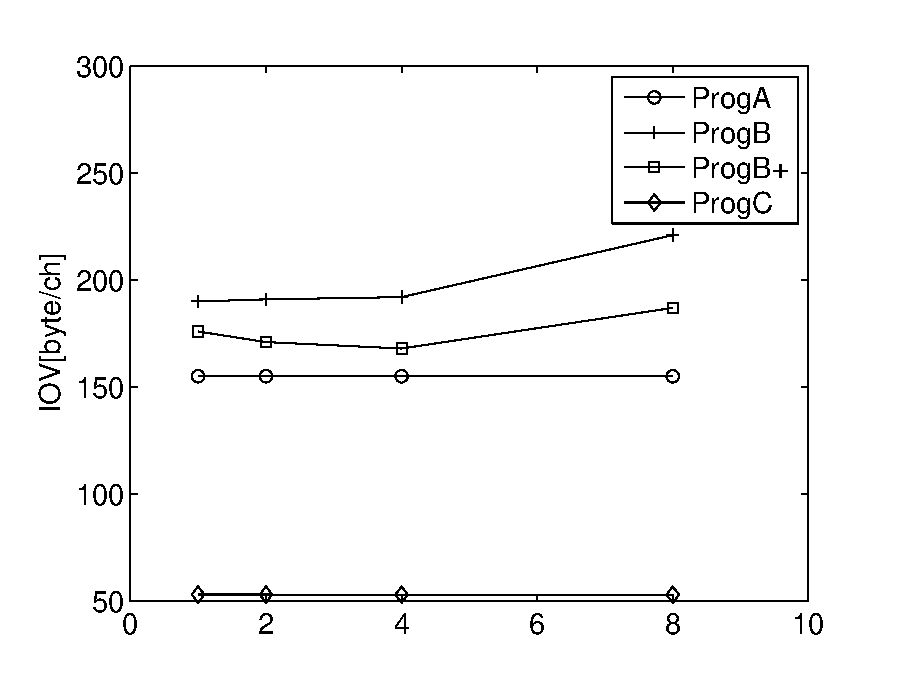
\includegraphics[width = 0.9\columnwidth]{io_cmp2}
	}
	\hfil
	\subfigure{
		\label{subfig:ct_cmp2}
		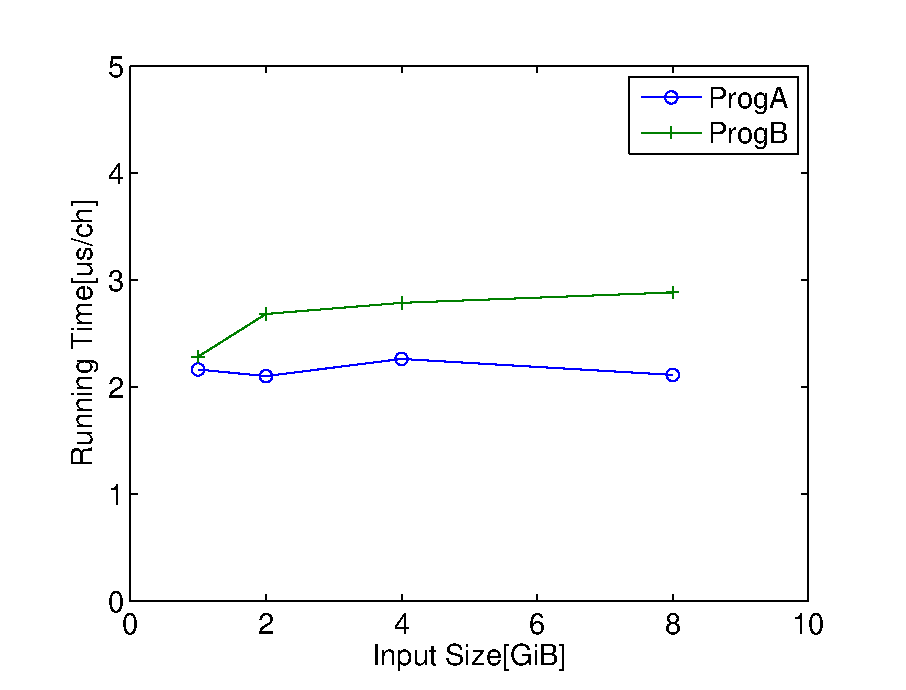
\includegraphics[width = 0.9\columnwidth]{ct_cmp2}
	}
	\caption{Performance of ProgA, ProgB, ProgB+ and ProgC for prefixes of "enwiki".}
	\label{fig:performance_analysis2}
\end{figure}
	
	
	
%Table
\renewcommand\arraystretch{1.3}
\begin{table*}
	\caption{A performance comparison of checking the suffix and LCP arrays of S*-type suffixes to checking that of all the suffixes.}
	\label{tbl:2}
	\centering
	\begin{tabular}{|l|c|c|c|c|c|c|c|c|c|c|c|c|}
		\hline
		\multirow{2}{*}{Dataset} & \multicolumn{3}{|c|}{\# of suffixes} & \multicolumn{3}{|c|}{PDU} & \multicolumn{3}{|c|}{IOV} & \multicolumn{3}{|c|}{RT} \\\cline{2-13}
						 & S*-type & all & ratio & S*-type & all & ratio & S*-type & all & ratio & S*-type & all & ratio \\\hline
		enwiki\_1g & 329810376 & 1073741824 & 0.31 & 15.67 & 40 & 0.39 & 89.94 & 155 & 0.58 & 1.05 & 1.70 & 0.62 \\\hline
		enwiki\_2g & 650901939 & 2147483648 & 0.30 & 15.41 & 40 & 0.39 & 89.18 & 155 & 0.58 & 1.22 & 1.85 & 0.66 \\\hline
		enwiki\_4g & 1301327878 & 4294967296 & 0.30 & 15.45 & 40 & 0.39 & 89.14 & 155 & 0.58 & 1.19 & 1.89 & 0.63 \\\hline
		enwiki\_8g & 2586471839 & 8589934592 & 0.30 & 15.35 & 40 & 0.38 & 88.80 & 155 & 0.57 & 1.33 & 2.14 & 0.62 \\\hline	
		uniprot & 829262945 & 3028811776 & 0.27 & 13.94 & 40 & 0.35 & 83.80 & 155 & 0.54 & 1.04 & 2.26 & 0.46 \\\hline
		proteins & 379092002 & 1184366592 & 0.32 & 16.21 & 40 & 0.41 & 92.29 & 155 & 0.60 & 1.14 & 1.85 & 0.62	\\\hline
		mean & 1012811163 & 3189156522 & 0.30 & 15.34 & 40 & 0.38 & 88.86 & 155 & 0.57 & 1.16 & 1.95 & 0.60 \\\hline
	\end{tabular}
\end{table*}

%It is identified that both programs heavily rely on the performance of the external memory sorter in use. A potential candidate for improving their speed is to adapt a GPU-based multi-way sorter~(e.g.,~\cite{Leischner2010, Davidson2012}) for sorting massive data using external memory. By the aid of these fast sorting algorithms, the throughputs of the programs are expected to nearly approach the I/O bandwidth. Besides, the first two steps of Algorithm~\ref{alg:1} are independent of each other and thus can be executed in parallel for acceleration. This technique can be also applied to check the suffix and LCP arrays of the LMS suffixes in Algorithm~\ref{alg:3}.

%Currently, for Algorithm~\ref{alg:3}, step 2 constitutes the space bottleneck. It is worthy of mentioning that this step produces a copy of the suffix and LCP array during the inducing and checking processes. Actually, given that $\Sigma$ is of a constant size and $sa/lcp$ are known already, we can simply scan the input $sa/lcp$ to perform the inducing process and compare each induced suffix/LCP value with that in the given $sa/lcp$ to perform the checking process, resulting in less space consumption. To the end, we must maintain a read pointer for each suffix/LCP bucket in $sa/lcp$ to scan elements in sequence.

Because there is no solution for checking both suffix and LCP arrays in the existing literature,  comparing the outputs of two builders could be a way for checking (even though it is not checking in the strict sense, for both outputs may be incorrect). In the next experiment, we compare our programs with two builders for suffix and LCP arrays as follows, where each of them combines an existing suffix sorter with an LCP builder:


\begin{itemize}
	\item Solution 1: Use eSAIS for building SA and the sequential version of Sparse-$\phi$~\cite{Karkkainen2016} for building LCP array.
	
	\item Solution 2: Use pSAscan~\cite{Karkkainen2015} for building SA and the parallel version of Sparse-$\phi$ for building LCP array.
\end{itemize}


We select these programs because they are currently the fastest suffix and LCP arrays builders available to us. A runtime breakdown of the programs for these solutions on the prefixes of "enwiki" is given in Table~\ref{tbl:3}. The program for Solution 2 is about two times faster than that for Solution 1 and twice as fast as ProgA, which is mainly due to the high speed of pSAscan in this experiment. However, it is worthy of pointing out that both pSAscan and Sparse-$\phi$ are of the time and I/O complexities proportional to $n^2/M$. This is much higher than eSAIS and our checking algorithms when $n$ increases, and thus poses a strict limitation to the scalability of Solution 2. As reported in~\cite{Karkkainen2015}, when $n$ is considerably greater than $M$, eSAIS is much more time and I/O efficient than pSAscan. In this experiment, pSAscan builds the SA for "enwiki\_8g" in time double as that for "enwiki\_1g". For big $n$, it is reasonable to compare the results of our programs with that of Solution 1.

%Table
\renewcommand\arraystretch{1.3}
\begin{table*}[h]
	\caption{A runtime comparison for the programs of two construction solutions and ours.}
	\label{tbl:3}
	\centering
	\begin{tabular}{|c|c|c|c|c|c|c|c|c|}
		\hline
		\multirow{2}{*}{Dataset} & \multicolumn{3}{|c|}{Solution 1} & \multicolumn{3}{c|}{Solution 2} & \multirow{2}{*}{ProgA} & \multirow{2}{*}{ProgB+} \\\cline{2-7}
		 & eSAIS & sequential sparse-$\phi$ & total & pSAscan & parallel sparse-$\phi$ & total & & \\\hline
		enwiki\_1g & 2.21 & 0.61 & 2.82 & 0.39 & 0.59 & 0.98 & 1.70 & 2.54 \\\hline
		enwiki\_2g & 2.63 & 0.53 & 3.16 & 0.47 & 0.53 & 1.00 & 1.84 & 2.51 \\\hline
		enwiki\_4g & 2.90 & 0.63 & 3.53 & 0.59 & 0.40 & 0.99 & 1.89 & 2.56 \\\hline
		enwiki\_8g & 3.02 & 0.63 & 3.65 & 0.83 & 0.45 & 1.28 & 2.13 & 2.79 \\\hline
	\end{tabular}
\end{table*}


Currently, the method described in~\cite{Burkhardt2003} is the only known in the literature for checking SA. Despite that it can check SA only, in order to give a rough image for the performance of our methods, we implement it by STXXL and compare our implementation with ProgA and ProgB/ProgB+ in Fig.~\ref{fig:performance_analysis} and \ref{fig:performance_analysis2}. This method and its program are denoted by "Method C" and "ProgC", respectively. ProgC is about two times faster than ProgA and three times faster than ProgB+, where the runtime is consistent with the I/O volume. This performance gap can be significantly narrowed by improving the algorithm and program designs of Methods A and B, using the techniques discussed below.


\subsection{Discussion} \label{sec:experiments:discussion}

\subsubsection{Improvement in Algorithm Design} \label{sec:experiments:discussion:improve_algorithm_design}

There are several ways to improve the algorithm designs of the proposed checking methods. First, Algorithm~\ref{alg:1} sorts the tuples of $ST_1/ST_1', ST_2/ST_2', ST_3/ST_3'$ in sequence. These sorting processes are independent and can be parallelized on computation platforms with multiple disks supporting parallel reads and writes. Second, Method B verifies the suffix and LCP arrays using the induced sorting principle. At the time of writing this paper, the existing IS algorithms are naturally sequential. Recently, we have been conducting a study to design parallel IS algorithms, this work will also help improve the design of Algorithm~\ref{alg:2}. Third, both methods A and B assume a constant or integer alphabet in this paper. However, in practice, an input string is commonly of a constant alphabet, e.g. 4 and 256 characters for genome and text, respectively. In this case, Method B can be improved for better time and space performance by inducing the final suffix and LCP arrays directly from $sa_S/lcp_S$ or $sa_L/lcp_L$, which consist of all the sorted S-type or L-type suffixes with their LCP-values and can be obtained as follows. Given the alphabet is constant, we first scan the input string once to get the statistics for buckets in the input suffix array. Without loss of generality, suppose that the S-type characters are less, we scan the suffix array once to get $sa_S/lcp_S$ by using the bucket statistics to on-the-fly determine a scanned suffix is S-type or not. Then we check $sa_S/lcp_S$ by using Algorithm~\ref{alg:1} and induce $sa'/lcp'$ from them. In this way, we avoid the two integer sorts in the current fashion of Method B for retrieving $sa^*/lcp^*$ and speed up the inducing process by nearly half as well.

\subsubsection{Improvement in Program Design} \label{sec:experiments:discussion:improve_program_design}

Our programs are coded for experimental study only, from engineering aspects, there is still a big margin for better implementation. For example, both ProgA and ProgB/ProgB+ consume long CPU time and large I/O volume for sorting data in external memory. We currently use the containers provided by STXXL to execute the sorting processes without designing a specific sorter optimized for our purpose. It is possible to speed up each sorting process by high-performance radix-sort GPU algorithms. Secondly, all our programs require a disk space significant more than what it is really needed. The main reason is the disk space for saving temporary data is not freed in time even if the data is not needed any more. This is an implementation issue due to STXXL in use, can be solved by storing the temporary data using multiple files and deleting each file immediately when it is obsolete. 
	
Several algorithms for induced sorting a suffix and/or LCP arrays were proposed these recent years \cite{Nong15,Nong14,Bingmann12}, with different methods for solving the key problem of retrieving the preceding character of a sorted suffix in the inducing process. A recent work \cite{Karkkainen2017} engineering these induced sorting methods with some implementation optimizing techniques achieves a significant improvement over the previous results. As reported, the peak disk use is around $8n$ for 40-bit integers. Because the induced sorting process is the performance bottleneck for Method B, it is reasonable to expect that a better engineering implementation of the method will yield a remarkable improvement in both time and space. An optimized engineering of our methods is out of the scope of this paper and will be addressed elsewhere.

\subsubsection{Miscellaneous}
	
Method A is more general than the other alternatives, it can be generalized to check the correctness of the lexical order and LCP values of any pairs of suffixes, this makes it possible for verifying any full or sparse suffix/LCP array of any order. On the other hand, Method B can only check suffix and LCP arrays, while Method C is specific for checking SA only. This feature of Method A makes it applicable to various scenarios. For example, a suffix/LCP array may be broken due to software or hardware malfunctions. If a backup is not available and it is time-consuming to rebuild the whole array, then we can locate the bad areas using Algorithm~\ref{alg:1} and restore the partial SA for each area by calling a sparse SA construction algorithm. Another example is to check the correctness of a sparse SA, in this case, the number of suffixes in a sparse SA is commonly much smaller than that in the full SA, Algorithm~\ref{alg:1} could be an efficient verification solution.

\section{Conclusions} \label{sec:conclusion}

Two methods are proposed here for probabilistically checking a pair of given suffix and LCP arrays. Theoretically, the external-memory algorithms designed by these methods have better time and I/O complexities compared to the existing fastest construction algorithms. Our experimental results indicate that the current programs for Algorithm~\ref{alg:2} designed by Method B run slower than that for Algorithm~\ref{alg:1} designed by Method A, but they are much more space efficient than the latter. We also show in Section~\ref{sec:experiment} that there still remains much room for improving the algorithm and program designs of the proposed methods. Particularly, our experimental program for Method A can be parallelized to achieve higher time performance, while that for method B can be further optimized for checking arrays of constant alphabets that are most common in practice.

The IS method has been applied to successfully design a number of suffix and LCP arrays construction algorithms. A recent work \cite{Karkkainen2017} reports that a careful engineering of the IS in external memory can build a suffix array using around $8n$ bytes for $n\le 2^{40}$, which is approaching $6n$ bytes for the IS in internal memory. Besides, it runs the fastest for large $n$ in the experiments therein. This convinces that the IS method could be a stand for developing potentially optimal solutions for building suffix/LCP arrays. We design here the algorithms for checking a pair of given suffix and LCP arrays. In another paper, we will come up with a solution for building and checking a suffix/LCP array simultaneously using the IS method. By this way, no additional checker is needed to be distributed with a suffix/LCP array builder using the IS method.



%\section*{Acknowledgment}
%The work of Y. Wu, G. Nong and L. B. Han were supported by the Guangzhou Science and Technology Program grant 201707010165 and the Project of DEGP grant 2014KTSCX007. {\color{red} %The work of W. H. Chan was supported by...}

% Bibliography
\bibliographystyle{IEEEtran}
\bibliography{IEEEabrv,bibfile}

\clearpage
\appendices
\section{Overview on the Induction Phase} \label{sec:appendix}

Notice that ${\sf suf}(i) < {\sf suf}(j)$ if (1) $x[i] < x[j]$ or (2) $x[i] = x[j]$ and ${\sf suf}(i + 1) < {\sf suf}(j + 1)$; otherwise, ${\sf suf}(i) > {\sf suf}(j)$. This observation is utilized by the IS algorithms to sort suffixes as follows:

\begin{enumerate}[S1]
	\item 
	Clear S-type sub-buckets in $sa$. Scan $sa^*$ leftward and insert each element into the current rightmost empty position in the corresponding S-type sub-bucket.
	
	\item 
	Clear L-type sub-buckets in $sa$ and insert $n - 1$ into the leftmost position in ${\sf sa\_bkt_L}(x[n - 1])$. Scan $sa$ rightward with $i$ increasing from $0$ to $n - 1$. For each scanned non-empty $sa[i]$ with $t[sa[i] - 1] = 0$, insert $sa[i] - 1$ into the current leftmost empty position in ${\sf sa\_bkt_L}(x[sa[i] - 1])$.
	
	\item
	Clear S-type sub-buckets in $sa$. Scan $sa$ leftward with $i$ decreasing from $n - 1$ to $0$. For each scanned non-empty $sa[i]$ with $t[sa[i] - 1] = 1$, insert $sa[i] - 1$ into the current rightmost empty position in ${\sf sa\_bkt_S}(x[sa[i] - 1])$.
	
\end{enumerate}

In brief, given $sa^*$, S1 inserts all the S*-type suffixes into $sa$ in their lexical order. Then, S2-S3 induce the order of L- and S-type suffixes from those already sorted in $sa$, respectively, where the relative order of two suffixes induced into the same sub-bucket matches their insertion order according to the rule stated above. To be more specific, we show in Fig.~\ref{fig:example2} a running example of the induction phase.

As depicted, the input string $x$ contains 6 S*-type suffixes sorted in line 3. When finished inserting the S*-type suffixes in lines 5-6, we first find the head of each L-type sub-bucket (marked by the symbol $\wedge$) and insert ${\sf suf}(13)$ into $sa$. Notice that ${\sf suf}(13)$ consists of only one character, it must be the smallest L-type suffixes starting with $1$. Thus, we put ${\sf suf}(13)$ into the leftmost position in ${\sf sa\_bkt_L}(1)$ in line 8. Then, we scan $sa$ from left to right for inducing the order of all the L-type suffixes. In lines 10-11, when visiting $sa[0] = 13$ (marked by the symbol $@$), we check the type array $t$ to find $x[12] = 2$ is L-type and hence insert ${\sf suf}(12)$ into the current leftmost empty position in ${\sf sa\_bkt_L}(2)$. Similarly, in lines 12-13, we visit the next scanned item $sa[1] = 11$ and see that $t[10] = 0$, thus we place ${\sf suf}(10)$ into the current head of ${\sf sa\_bkt_L}(3)$. Following this way, we get all the L-type suffixes sorted in $sa$. After that, we first find the end of each S-type sub-bucket in lines 25-26 and scan $sa$ leftward for inducing the order of all the S-type suffixes in lines 27-40. When visiting $sa[13] = 2$, we see $x[1]$ is S-type and thus put ${\sf suf}(1)$ into the current rightmost empty position in ${\sf sa\_bkt_S}(1)$. Then, at $sa[12] = 8$, we see $x[7] = 1$ is S-type and thus put ${\sf suf}(7)$ into the current rightmost empty position in ${\sf sa\_bkt_S}(1)$. To repeat scanning $sa$ in this way, we get all the S-type suffixes sorted in $sa$. 

The work in~\cite{Fischer11} describes how to compute the LCP array during the execution of S2-S3. Given two suffixes placed at the neighboring positions in $sa$, their LCP-value can be computed according to one of the following two cases in respect to whether or not they are inserted into the same sub-bucket: if yes, then their LCP-value is one greater than that of the two suffixes from which inducing them; otherwise, their LCP-value equals to zero. In this way, we can determine $lcp[i]$ immediately after the computation of $sa[i]$. The problem here is how to obtain the LCP-values of these inducing suffixes starting at the next positions in $x$, which is modeled as a range minimum query in~\cite{Fischer11} and can be answered within amortized $\mathcal{O}(1)$ time. For example, when scanning $sa[0]$ and $sa[5]$ in lines 10-11 and 20-21 of Fig.~\ref{fig:example2}, ${\sf suf}(12)$ and ${\sf suf}(6)$ are sequentially induced into the neighboring positions in ${\sf sa\_bkt_L(2)}$. In the meantime, if we keep recording the minimum over $lcp(0, 5]$, then we can obtain the LCP-value of the inducing suffixes ${\sf suf}(13)$ and ${\sf suf}(7)$ when putting the induced suffix ${\sf suf}(6)$ into $sa$.

\begin{figure}
	\centering
	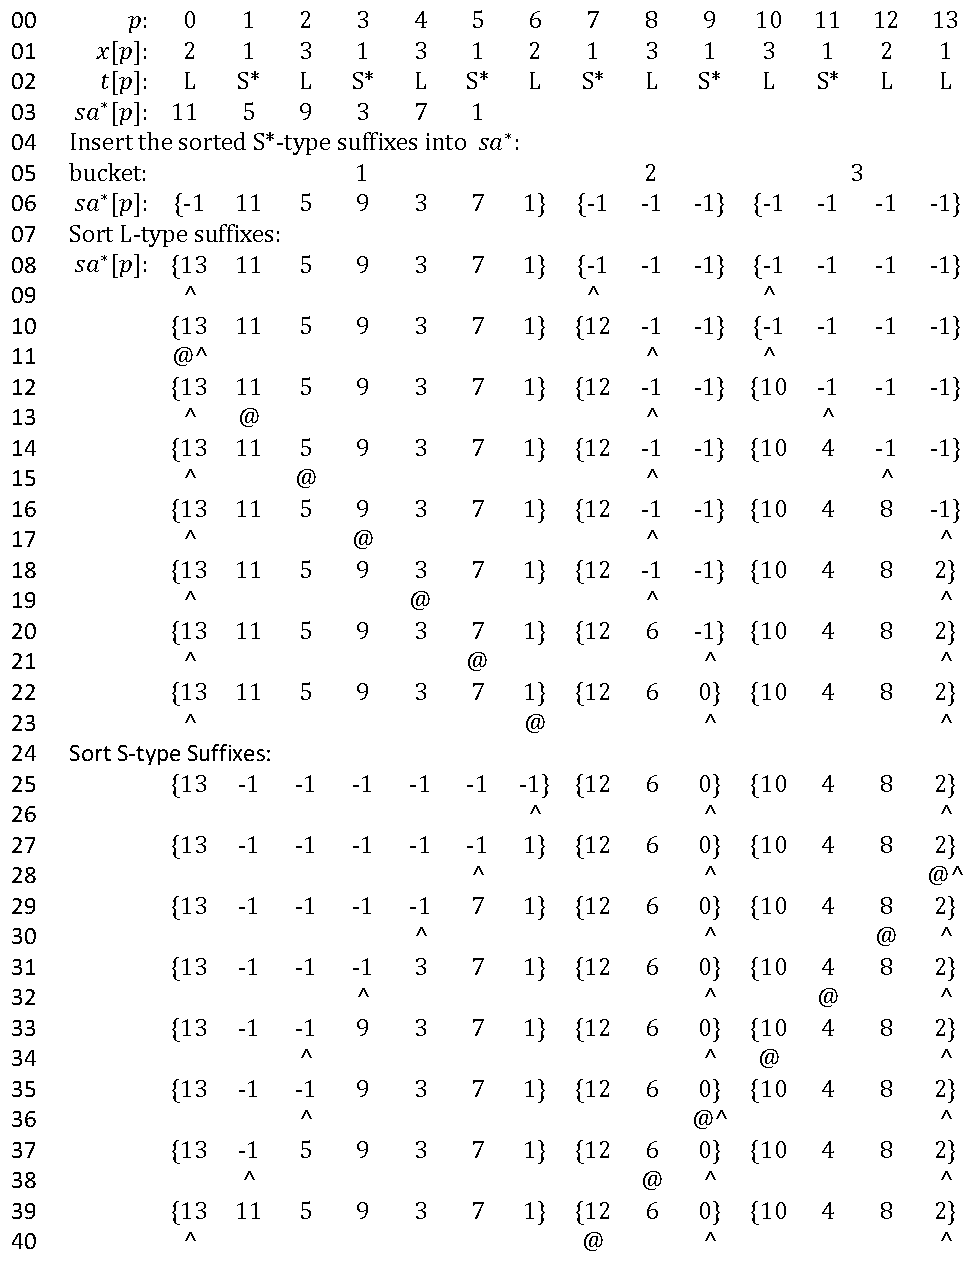
\includegraphics[width = 0.9\columnwidth]{example2}

	\caption{An Example for inducing the suffix and LCP arrays. \label{fig:example2}}	
\end{figure}
 
	
\end{document}






























